\section{序論}
hikiは,hiki記法を用いたwiki cloneである.wikiはウォード・カニンガムが作ったwikiwikiwebを源流とするhome page制作を容易にするシステムで,hikiもwikiの基本要求仕様を満足するシステムを提供する.wikiの特徴であるweb上で編集する機能を提供する.これを便宜上hiki web systemと呼ぶ.図にある通り,一般的な表示画面の他に,編集画面が提供されており,ユーザーはこの編集画面からコンテンツを編集することが可能である.リンクやヘッダー,リスト,引用,表,図の表示などの基本テキストフォーマットが用意されている.
\begin{quote}\begin{verbatim}
hiki web systemの実際の基本動作は,hiki.cgiプログラムを介して行われている.こちらを便宜上hiki systemと呼ぶ.図に従ってhiki systemの動作概要を説明する.hiki systemは,data/textに置かれた書かれたプレーンテキストをhtmlへ変換する.この変換はhikidoc[1]というhikiフォーマットconverterを使っている.また,添付書類はcache/attachに,一度フォーマットしたhtmlはparserに置かれており,それらを参照してhtmlを表示する画面をhiki.cgiは作っている.さらにhiki systemでは検索機能,自動リンク作成などが提供されている
=======
hiki web systemの実際の基本動作は,hiki.cgiプログラムを介して行われている.こちらを便宜上hiki systemと呼ぶ.図{{ref(fig:one)}}に従ってhiki systemの動作概要を説明する.hiki systemは,data/textに置かれた書かれたプレーンテキストをhtmlへ変換する.この変換はhikidoc{{cite(1-1)}}というhikiフォーマットconverterを使っている.また,添付書類はcache/attachに,一度フォーマットしたhtmlはparserに置かれており,それらを参照してhtmlを表示する画面をhiki.cgiは作っている.さらにhiki systemでは検索機能,自動リンク作成などが提供されている
\end{verbatim}\end{quote}
\begin{figure}[htbp]\begin{center}
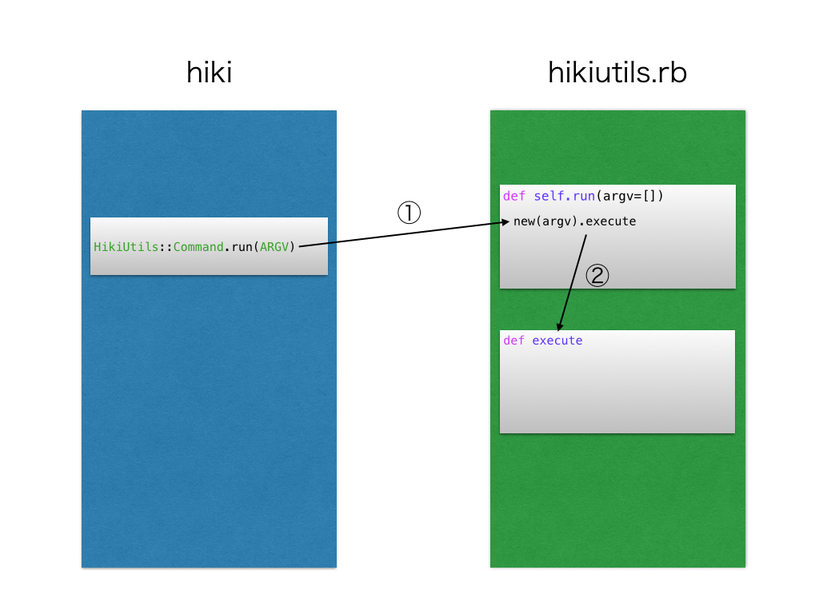
\includegraphics[width=10cm,bb= 0 0 737 553]{../figs/./hikiutils_yamane.001.jpg}
\caption{hiki web systemとhiki systemの対応関係.}
\label{fig:one}
\label{default}\end{center}\end{figure}
研究室内の内部文書,あるいは外部への宣伝資料,さらにwikipediaのように重要な研究成果の発信などに西谷研ではこのhiki systemを利用している.初心者にも覚えやすい直感的な操作である.しかし,慣れてくるとテキスト編集や画面更新にいちいちweb画面へ移行せねばならず,編集の思考が停止する.そこで,テキスト編集に優れたeditorとの連携や,terminal上のshell commandと連携しやすいようにhikiutilsというCLI(Command Line Interface)を作成して運用している.しかし,そのユーザインタフェースにはコマンドが直感的でないという問題点がある.そこで,Thorというコマンドラインツール作成ライブラリを用いる.hikiutilsでは,optparseというコマンドライン解析ライブラリを使用しているが,新たなライブラリThorを使用してコマンドを書き換え,より直感的なコマンドに変更する.

